\autoref{fig:bearing_fh_tm} shows, that the \ac{TM} can be positioned at various distances and angles in relation to the \ac{FH}.
For one corn harvest scenario, \textcite{klingler_agriculture_2018} found out, that the \ac{RSS} can drop due to
shadowing effects caused by the size and shape of the \ac{FH} and the \ac{TM}.

In a field experiment, I want to analyze which positions of the \ac{TM} and \ac{FH} cause the shadowing effects, which
subsequently reduce the \ac{RSS} and how physical layer parameters like \ac{MCS} and \ac{STBC} can used to ensure a low
\ac{PER}.

For the experiment, I will use a \ac{CH} instead of a \ac{FH} as it has a similar shape and size as a \ac{FH} and is available.
The \ac{TM} will be a Tractor pulling a trailer of the type HW80.
Both machines will be equipped with a \ac{GPS} receiver and Wi-Fi devices which record the \ac{RSS} and the \ac{PER} of the
exchanged packets.
The \ac{CH} will be positioned on a field.
The tractor will start \SI{50}{\metre} behind the \ac{CH}, advance to the \ac{CH} and pass the \ac{CH} slowly with a
speed of \SIrange{1}{10}{\kilo\metre\per\hour} as shown in \autoref{fig:fieldDrive}.
\begin{figure}[]%
	\centering
	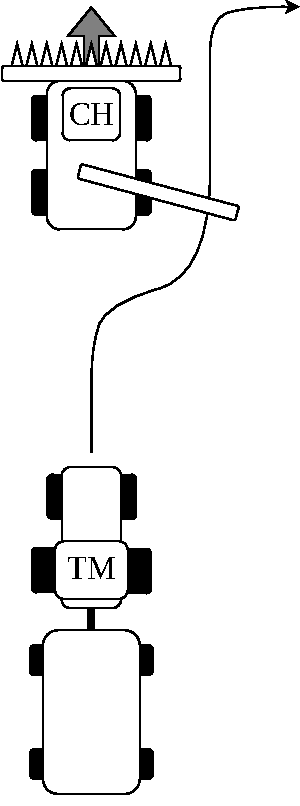
\includegraphics[width=0.4\textwidth]{figures/FieldExperimentDrive}
	\caption{Path around the static \acf{CH}, which the \acf{TM} will drive during the experiment to mimic various overloading positions}%
\end{figure}
Thereby, the tractor will mimic various the overloading positions, where shadowing effects can occur. After the tractor has passed the \ac{CH},
it will drive back to its starting position and the experiment will be repeated with different overloading distances between the \ac{CH} and the tractor.

During the experiments the \ac{GPS} receivers at the agricultural machines will record the position and speed of the machines every \SI{1}{\second}.

The Wi-Fi setup consists of a Milesight Industrial Router UR75 which is mounted on the roof of the tractor at a height \SI{4}{\metre} above the ground.
\textcite{brinkhoff_characterization_2017} and \textcite{paul_characterizing_2011}  already found out, that placing the antenna higher above ground improves
the robustness and communication range of Wi-Fi networks in an outdoor environment. As the regulation in StVZO §32 Abs. 2  limits the height of
every agricultural vehicle or combination of vehicles to less than \SI{4.0}{\metre}, the maximum antenna is \SI{4}{\metre} above the ground.

Additionally, two UP Squared Board are equipped with a Intel AX210 Wi-Fi module each, which is connected two antennas each. The
antennas support omnidirectional transmissions in the \SI{2.4}{\giga\hertz}, \SI{5}{\giga\hertz} and \SI{6}{\giga\hertz} band and have a gain of \SI{5}{\decibel}.
The boards are mounted on the roof of the \ac{CH} at a height \SI{4}{\metre} above the ground.

The router on the tractor sets up a Wi-Fi \ac{AP} in the \SI{5.6}{\giga\hertz} band, which can be used for outdoor Wi-Fi transmissions \cite{freq_plan}.One of the boards on the \ac{CH} connects to the \ac{AP} of the router as a Wi-Fi \ac{STA} and hosts an iperf3 \footnote{https://iperf.fr/ Accessed: 8.3.2023} server.
A notebook is connected via LAN to the router and runs an iperf3 client, which connects to the iperf3 server on the \ac{CH}.
The iperf3 client sends \SI{1000}{\byte} UDP packets every second to the iperf3 server on the \ac{CH}. The server records the received packets and
send an acknowledgement back to the client. The recorded received packets are used to calculate the \ac{PER} of the transmitted packets.

The other board on the \ac{CH} uses the Wi-Fi card in the monitor mode and records every transmission in the \SI{5.6}{\giga\hertz} band using tcpdump \footnote{https://www.tcpdump.org/ Accessed: 8.3.2023}.
Tcpdump records every transmitted frame in pcap format, which can be analyzed using Wireshark\footnote{https://www.wireshark.org/ Accessed: 8.3.2023}.
The transmissions are displayed in \autoref{fig:fieldWifi}.
\begin{figure}[]%
	\centering
	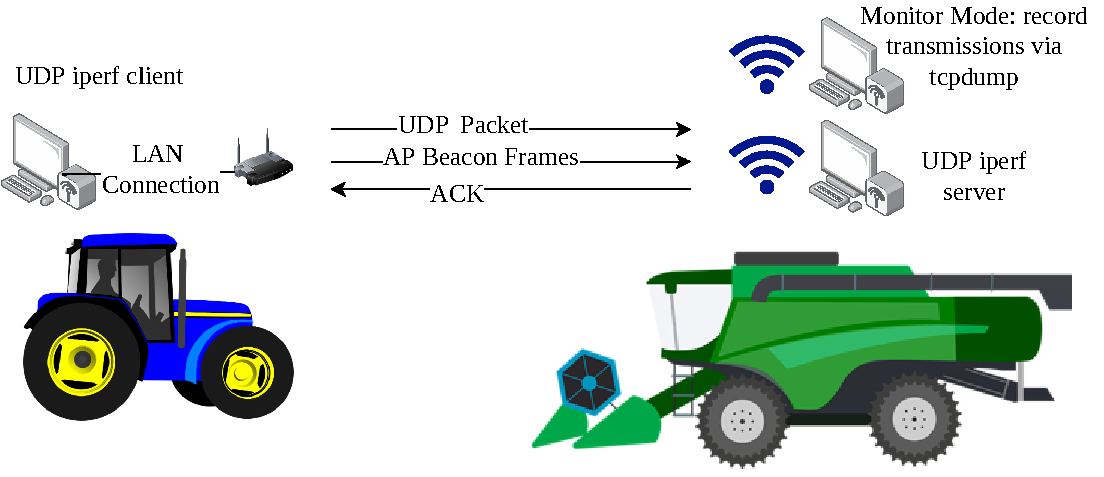
\includegraphics[width=0.8\textwidth]{figures/FieldExperimentwifi}
	\caption{Simulated \ac{PER} in regards to \ac{SNR} for chosen HE-\ac{MCS} values and whether \ac{DCM} is enabled for IEEE 802.11ax physical layer parameters of a \ac{GI} of \SI{3200}{\nano\second}, a \ac{BW} of \SI{20}{\mega\hertz} and 2 spatial streams}%
	\label{fig:fieldWifi}%
\end{figure}
Among other information, the recorded pcap files contain the \ac{RSS} of every antenna and the \ac{PER} of the transmitted packets.